\documentclass{beamer}

\usepackage{beamerthemesplit}
\usepackage{graphicx}
\usepackage{color, natbib, hyperref}

% define colors
\definecolor{jblue}  {RGB}{20,50,100}
\definecolor{ngreen} {RGB}{98,158,31}

%theme

\usetheme{boxes} 
%\usecolortheme{seahorse} 
\setbeamertemplate{items}[default] 
%\setbeamercovered{transparent}
\setbeamertemplate{blocks}[rounded][shadow=true] 
\setbeamertemplate{navigation symbols}{} 
% set the basic colors
\setbeamercolor{palette primary}   {fg=black,bg=white}
\setbeamercolor{palette secondary} {fg=black,bg=white}
\setbeamercolor{palette tertiary}  {bg=jblue,fg=white}
\setbeamercolor{palette quaternary}{fg=black,bg=white}
\setbeamercolor{structure}{fg=jblue}
\setbeamercolor{titlelike}         {bg=jblue,fg=white}
\setbeamercolor{frametitle}        {bg=jblue!10,fg=jblue}
\setbeamercolor{cboxb}{fg=black,bg=jblue}
\setbeamercolor{cboxr}{fg=black,bg=red}

% set colors for itemize/enumerate
\setbeamercolor{item}{fg=ngreen}
\setbeamercolor{item projected}{fg=white,bg=ngreen}

% set colors for blocks
\setbeamercolor{block title}{fg=ngreen,bg=white}
\setbeamercolor{block body}{fg=black,bg=white}

% set colors for alerted blocks (blocks with frame)
%\setbeamercolor{block alerted title}{fg=white,bg=jblue}
%\setbeamercolor{block alerted body}{fg=black,bg=jblue!10}
\setbeamercolor{block alerted title}{fg=white,bg=dblue!70} % Colors of the highlighted block titles
\setbeamercolor{block alerted body}{fg=black,bg=dblue!10} % Colors of the body of highlighted blocks

% set the fonts
\usefonttheme{professionalfonts}

\setbeamerfont{section in head/foot}{series=\bfseries}
\setbeamerfont{block title}{series=\bfseries}
\setbeamerfont{block alerted title}{series=\bfseries}
\setbeamerfont{frametitle}{series=\bfseries}
\setbeamerfont{frametitle}{size=\Large}
\setbeamerfont{block body}{series=\rmfamily}
\setbeamerfont{caption}{series=\rmfamily}
\setbeamerfont{headline}{series=\rmfamily}


% set some beamer theme options
\setbeamertemplate{title page}[default][colsep=-4bp,rounded=true]
\setbeamertemplate{sections/subsections in toc}[square]
\setbeamertemplate{items}[circle]
\setbeamertemplate{blocks}[width=0.0]
\beamertemplatenavigationsymbolsempty

\mode<presentation>

\title[Model-based matching]{Model-based matching for causal inference in observational studies}
\author{Kellie Ottoboni}
\institute[]{Department of Statistics, UC Berkeley}
\date{\today}

\begin{document}

\frame{\titlepage}

\frame
{
  \frametitle{Observational Studies vs Experiments}
 \begin{center}
\begin{itemize}
\item In randomized control trials, treatment is assigned to individuals at random.
\item In observational studies, the way individuals select into treatment groups is unknown.
\item \textbf{Confounding} occurs when a variable affects both treatment assignment and the outcome. It biases our estimates of the treatment effect.
\end{itemize}
\end{center}
}


\frame
{
  \frametitle{Matching}
\begin{center}
\begin{itemize}
\item \textbf{Ideal:} group individuals by important confounders to estimate subgroup treatment effects and then average over subgroups
\item \textbf{Reality:} many covariates, perhaps continuous, make it difficult to stratify
\item \textbf{Solution:} use a one-dimensional score to match or group individuals
\item  Stratify according to the ``best'' prediction of the response, based on all covariates except for the treatment
\end{itemize}
\end{center}
}

\frame
{
  \frametitle{Model-based Matching}
\begin{center}
\begin{itemize}
\item Under standard assumptions (conditional independence of treatment and potential outcomes given $X$), the \textbf{average treatment effect} is nonparametrically identified
\item Estimate it using the difference in average residuals between treated and controls
\end{itemize}

\begin{figure}[htbp]
\begin{center}
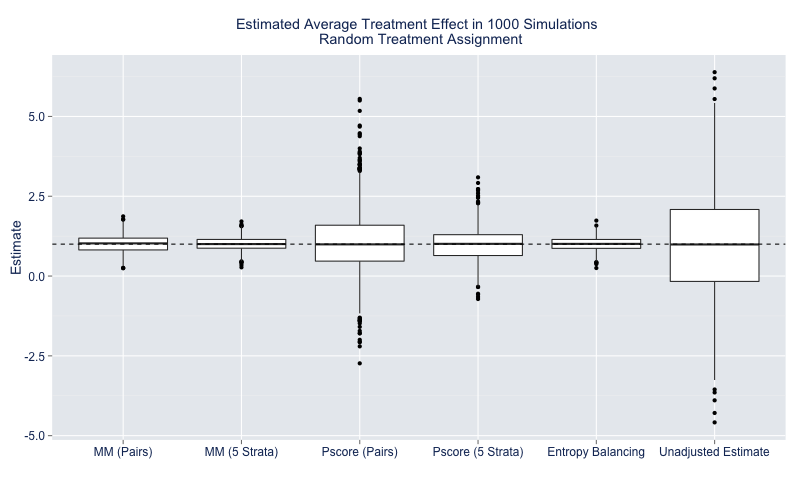
\includegraphics[width = 0.9\textwidth]{fig/estimates.png}

\end{center}
\end{figure}


\end{center}
}

\frame
{
  \frametitle{Model-based Matching}
\begin{center}
\begin{itemize}
\item Use stratified permutation test to test the \textbf{strong null hypothesis} of no treatment effect whatsoever
\item Stratifying on $\hat{Y}$ allows us to detect non-constant and non-linear treatment effects
\end{itemize}

\begin{figure}[htbp]
\begin{center}
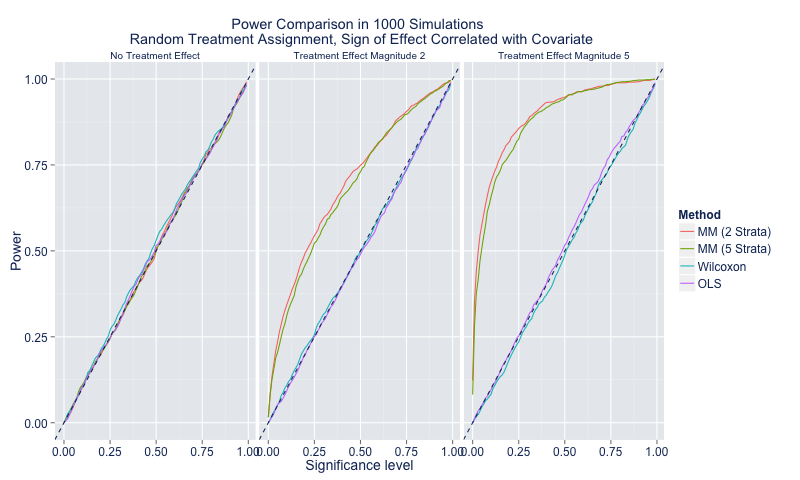
\includegraphics[width = 0.9\textwidth]{fig/power.png}
\end{center}
\end{figure}


\end{center}
}

\frame
{
  \frametitle{Future Directions}
\begin{center}
\begin{itemize}
\item Do different test statistics give greater power when the treatment effect is nonlinear?
\item What is the optimal way to stratify?
\item How to quantify uncertainty -- standard errors and confidence intervals?
\end{itemize}
\end{center}
}



%
%\section{References}
%\begin{frame}
%\frametitle{References}
%\bibliographystyle{plainnat}
%\bibliography{refs}
%\itemize
%\end{frame}

\end{document}
